% Section 04 - Inverse Scattering Time Analysis

The Floquet-Fermi golden rule was proposed in Ref. \cite{wackerl20} as an approach to analyze the transport properties of dressed quantum systems with impurities.
However, this theory has not been applied for a dressed quantum Hall system in the previous studies. In this analysis, we use Floquet-Fermi golden rule to identify the effects induced by impurities on the magneto-transport properties.
With the help of $t-t'$ formalism \cite{wackerl20,grifoni98,sambe75,peskin93,althorpe97} and applying Floquet states derived in Eq.~(\ref{eq:14}), we can derive an  expression for $(l,l')$-th element of the inverse scattering time matrix for the $N$-th Landau level as
\begin{widetext}
\begin{equation} \label{eq:15}
  \begin{aligned}
    \left(\frac{1}{\tau(\varepsilon,k_x)}\right)^{ll'}_N = &
    \frac{ \varrho^2}{eB} \delta(\varepsilon - \varepsilon_N) \\
    & \times
    \int_{-\infty}^{\infty}
    J_l \bm{\left(} \frac{b\hbar}{eB}({k}_x - k_1) \bm{\right)}
    J_{l'} \bm{\left(} \frac{b\hbar}{eB}({k}_x - k_1) \bm{\right)}
    \left|
    \int_{-\infty}^{\infty}
    \chi_N \left( \frac{\hbar}{eB}k_2 \right)
    \chi_N \bm{\left(} \frac{\hbar}{eB}
    \left( k_1 - {k}_x - k_2 \right) \bm{\right)}
    dk_2 \right|^2 d k_1,
  \end{aligned}
\end{equation}
\end{widetext}
where $\varrho = \eta_{imp} L_x \left[\flatfrac{ V_{imp}}{(eB)}\right]^{1/2}$, $\varepsilon$ is a given energy value, $J_l(\cdot)$ are Bessel functions of the first kind with $l$-th integer order, and $\varepsilon_N$ is the energy of the $N$-th Landau level.
A more detailed derivation is given in Appendix \ref{appendix_c}.
We modeled the effect caused by impurities in the considered system as a single perturbation potential.
Since random impurities in a disordered metal offer a better approximation for experimental conditions, we assumed that our perturbation potential is formed by a group of randomly distributed impurities.
Thus, the total scattering potential in the 2DEG has been represented as a sum of uncorrelated single impurity potentials $\upsilon(\vb{r})$. Here $\eta_{imp}$ is the number of impurities in a unit area, $V_{imp} = \expval{|V_{{k'}_x,k_x}|^2}_{imp}$ with $V_{{k'}_x,k_x} = \mel**{k'_x}{\upsilon(x) }{k_x}$, and $\braket{x}{k_x} = e^{-ik_x x}$.
Moreover, in this analysis, $\expval{\cdot}_{imp}$ represents the average over the impurity disorder.

Next, we analyze the contribution of the inverse scattering time matrix elements on the transport properties of our system.
Since the disorder in the system can not significantly alter the eigenenergy values of the undressed system \cite{wackerl20}, we can neglect the contribution of all off-diagonal elements in the inverse scattering time matrix. Subsequently we consider only the central diagonal element (${l=l'=0}$) of the inverse scattering time matrix which has the largest contribution to the transport characteristics. Along with this assumption, we introduce a new parameter as the scattering-induced broadening of the $N$-th Landau level \cite{dini16,endo09}
\begin{equation} \label{eq:16}
 \Gamma^{00}_{N}(\varepsilon,k_x) =
 \hbar \left(\frac{1}{\tau(\varepsilon,k_x)}\right)^{00}_N,
\end{equation}
which simplifies to
\begin{widetext}
  \begin{equation} \label{eq:17}
   \begin{aligned}
     &\Gamma^{00}_{N} (\varepsilon,k_x) =
     \frac { \varrho^2}{eB}
     \delta(\varepsilon - \varepsilon_{N})
     \int_{-\infty}^{\infty}
     J_0^2 \bm{\left(} \frac{b\hbar}{eB}({k}_x - k_1) \bm{\right)}
     \left|
     \int_{-\infty}^{\infty}
     \chi_N \left( \frac{\hbar}{eB}k_2 \right)
     \chi_N \bm{\left(} \frac{\hbar}{eB}
     \left( k_1 - {k}_x - k_2 \right) \bm{\right)}
     dk_2 \right|^2 d k_1.
   \end{aligned}
  \end{equation}
In addition, for a scattering scenario taking place within the same Landau level, we are able to present the delta distribution of the energy by the  interpretation \cite{dini16}
\begin{equation} \label{eq:18}
 \delta(\varepsilon - \varepsilon_{N}) \approx
 \frac{1}{\pi \Gamma^{00}_N (\varepsilon,k_x)}.
\end{equation}
Then we write the central element of inverse scattering time matrix in the more compact form
\begin{equation} \label{eq:19}
  \begin{aligned}
    &\Gamma^{00}_{N}(\varepsilon,k_x) =
     \varrho
      \left[
      \int_{-\infty}^{\infty}
      J_0^2 \bm{\left(} \lambda_1 (k_x - k_1) \bm{\right)}
      \left|
      \int_{-\infty}^{\infty}
      \widetilde{\chi}_{N}\left(\lambda_2 k_2 \right)
      \widetilde{\chi}_{N} \bm{\left(} \lambda_2 (k_1 - k_2 - k_x) \bm{\right)}
      dk_2 \right|^2
      dk_1
      \right]^{-\frac{1}{2}},
  \end{aligned}
\end{equation}
where $ \lambda_1 = \flatfrac{\hbar b}{(eB)}$ and  $\lambda_2 = \flatfrac{\hbar \kappa}{(eB)}$.
To analyze the effects of the dressing field on the scattering-induced broadening, we introduce the normalized $N$-th Landau level scattering-induced broadening as
\begin{equation} \label{eq:20}
    \Lambda_N(k_x) =
    \frac{\Gamma^{00}_N (\varepsilon,k_x)}
    {\Gamma^{00}_{N=0}(\varepsilon,k_x)\big|_{E=0}},
\end{equation}
which can be evaluated with
\begin{equation} \label{eq:21}
    \Lambda_N (k_x) =
    \left[
    \frac
    {
      \int_{-\infty}^{\infty}
      J_0^2 \bm{\left(} \lambda_1 (k_x - k_1) \bm{\right)}
      \left|
      \int_{-\infty}^{\infty}
      \widetilde{\chi}_{N}\left(\lambda_2 k_2 \right)
      \widetilde{\chi}_{N} \bm{\left(} \lambda_2 (k_1 - k_2 - k_x) \bm{\right)}
      dk_2 \right|^2
      dk_1
    }
    {
      \int_{-\infty}^{\infty}
      \left|
      \int_{-\infty}^{\infty}
      \widetilde{\chi}_0 \left(\lambda_2 k_2 \right)
      \widetilde{\chi}_0 \bm{\left(} \lambda_2 (k_1 - k_2 - k_x) \bm{\right)}
      dk_2 \right|^2
      dk_1
    }
    \right]^{1/2}.
\end{equation}
\end{widetext}

\begin{figure}[h!]
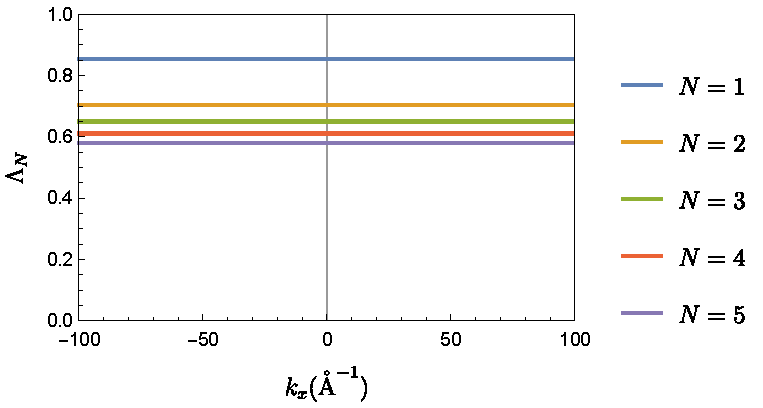
\includegraphics[scale=0.68]{figures/fig_2}
\caption{\label{fig_3} The dependence of normalized scattering-induced broadening $\Lambda_N$ for each Landau level ($N =0,1,2,3,4$) against $x$-directional momentum value $k_x$ in a GaAs-based quantum well under a nonoscillating magnetic field with $B = \SI{1.2}{\tesla}$, dressing field with a  frequency of $\omega =\SI{2e12}{\radian\per\second}$ and intensity $I =\SI{100}{\watt\per\square\centi\metre}$.
In this calculation, we have assumed that the natural  broadening of $0$-th Landau level $\Gamma_0$ is $\SI{0.24}{\milli\eV}$.}
\end{figure}
\begin{figure}[t!]
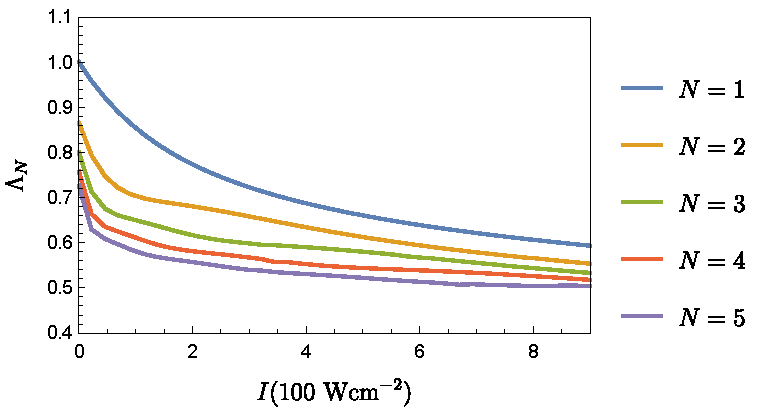
\includegraphics[scale=0.68]{figures/fig_3}
\caption{\label{fig_4} The dependence of normalized scattering-induced broadening $\Lambda_N$ for each Landau level ($N =0,1,2,3,4$) against dressing field intensity $I$, in a GaAs-based quantum well under a nonoscillating magnetic field with $B = \SI{1.2}{\tesla}$, dressing field with a frequency of $\omega =\SI{2e12}{\radian\per\second}$. In this calculation, we have assumed that the natural broadening of $0$-th Landau level $\Gamma_0$ is $\SI{0.24}{\milli\eV}$.}
\end{figure}

Normalized energy band broadening against $x$-directional momentum component ${k_x}$ for different Landau levels ($N = 0,1,2,3,4$) has been calculated for GaAs-based quantum well and the results are depicted in Fig.~(\ref{fig_3}) and Fig.~(\ref{fig_4}). To make a comparison, we have selected the experiment parameters to match with analysis in Ref.~\cite{endo09}.
In that study, the authors have assumed that the effective mass of the electron in GaAs-based quantum well system is $m_e \approx 0.07\widetilde{m}_e$ where $\widetilde{m}_e$ is the mass of the electron \cite{endo09,winkler03,wackerl20}. In addition, they used the broadening of the undressed $0$-th Landau level $\Gamma_0$ as $\SI{0.24}{\milli\eV}$. Therefore, in our calculations, we assumed that the natural least Landau level broadening also has this value: $\Gamma^{00}_{N=0}|_{E=0} = \SI{0.24}{\milli\eV}$.
Here, we observe that the normalized energy broadening value for each Landau level is independent of the $x$-directional momentum $k_x$ value and we are able to manipulate it by the dressing field. When the dressing field's intensity increases, the energy broadening is reduced, which leads to changes in the transport properties of the dressed quantum Hall system.
To analyze these adjustments in detail, we derive an analytical expression for the conductivity of a dressed quantum Hall system in the next section.
